\documentclass[12pt]{article}
\usepackage{../../format}
\lhead{A Level Physics}
\setcounter{secnumdepth}{5}
\usepackage[english]{babel}

\makeatletter
\renewcommand{\paragraph}{\@startsection{paragraph}{4}{0ex}%
    {-3.25ex plus -1ex minus -0.2ex}%
    {1.5ex plus 0.2ex}%
    {\normalfont\normalsize\bfseries}}
\makeatother

\begin{document}
\begin{center}
\underline{\huge Paper 1 Cheat Sheet}
\end{center}
\section{Measurements and their errors}
\textbf{Precision} - There is very little spread around the mean value\\
\textbf{Repeatability} - If the same experimenter repeats the investigation using the same method and equipment and obtains the same results\\
\textbf{Reproducibility} - If a different experimenter repeats the investigation, or uses a different experiment or technique, the same results are obtained\\
\textbf{Accuracy} - Close to the true value\\
{\renewcommand{\arraystretch}{2}
\begin{tabularx}{\textwidth}{|X|X|}
\hline
Combination&Operation\\
\hline
Adding or subtracting\newline $a=b+c$&Add the absolute uncertainties\newline $\Delta a=\Delta b+\Delta c$\\
\hline
Multiplying values\newline $a=b\times c$&Add the percentage uncertainties\newline $\epsilon a=\epsilon b+\epsilon c$\\
\hline
Dividing values\newline $a=\dfrac{b}{c}$&Add the percentage uncertainties\newline $\epsilon a=\epsilon b+\epsilon c$\\
\hline
Power rules\newline $a=b^c$&Multiply the percentage uncertainty by the power\newline $\epsilon a=c\times\epsilon b$\\
\hline
\end{tabularx}}
\newpage
\section{Particles and radiation}
\subsection{Constituents of the atom}
Protons and neurons in the centre, with shells of electrons around them
$$\textrm{Specific charge}=\frac{Q}{m}$$
\textbf{Isotope} - An atom with the same number of protons and electrons as an element, but a different number of neutrons
\subsection{Stable and unstable nuclei}
\subsubsection{The strong nuclear force}
\begin{tabular}{|c|c|}
\hline
$<0.5fm$&Repulsion\\
\hline
$0.5-3fm$&Attraction\\
\hline
$3fm+$&No force\\
\hline
\end{tabular}
\subsubsection{Alpha decay}
{\large
$$^A_ZX\rightarrow ^{A-4}_{Z-2}Y+^4_2\alpha$$
\subsubsection{Beta decay}
$$^A_ZX\rightarrow ^A_{Z+1}+^0_{-1}\beta+\overline{\nu}$$}
Neutrinos were hypothesised to allow for energy to be conserved in the interaction
\subsection{Particles, antiparticles and photons}
\subsubsection{Particle antiparticle pairs and their properties}
{\def\arraystretch{1.5}
\begin{tabularx}{\textwidth}{|X|X|X|}
\hline
\textbf{Property}&\textbf{Particle}&\textbf{Antiparticle}\\
\hline
Mass&x&x\\
\hline
\textcolor{red}{Charge}&x&-x\\
\hline
Rest Energy&x&x\\
\hline
\textcolor{red}{Baryon Number}&x&-x\\
\hline
\textcolor{red}{Lepton Number}&x&-x\\
\hline
\textcolor{red}{Strangeness}&x&-x\\
\hline
\end{tabularx}}
\newpage
\paragraph{Mesons}
\subparagraph{Pions(All 0 Strangeness)}
$ $\\
{\def\arraystretch{1.5}
\begin{tabularx}{\textwidth}{|X|X|}
\hline
$\pi^0$&$U\bar{U}$ or $D\bar{D}$\\
\hline
$\pi^+$&$U\bar{D}$\\
\hline
$\pi^-$&$D\bar{U}$\\
\hline
\end{tabularx}}
\subparagraph{Kaons (All strange)}
$ $\\
{\def\arraystretch{1.5}
\begin{tabularx}{\textwidth}{|X|X|}
\hline
$K^+$&$U\bar{S}$\\
\hline
$K^-$&$\bar{U}S$\\
\hline
$K^0$&$D\bar{S}$\\
\hline
$\bar{K^0}$&$\bar{D}S$\\
\hline
\end{tabularx}}
\subsubsection{The photon model of electromagnetic radiation}
A photon is a particle whose energy depends on its frequency. Formulas can be found on the data sheet to calculate this relationship
\subsubsection{Methods of annihilation and pair production}
\paragraph{Annihilation}
When a particle and an antiparticle meet, they annihilate each other, releasing two photons, with energy sum equivalent to the sum of the energy of the particle and antiparticle. This energy can be calculated from the rest energy values on the data sheet.
$$hf_{min}=E_0$$
\paragraph{Pair production}
In pair production a photon creates a particle and an antiparticle
$$hf_{min}=2E_0$$
\subsection{Particle interactions}
\subsubsection{The four fundamental interactions}
{\def\arraystretch{1.5}
\begin{tabularx}{\textwidth}{|X|X|X|X|}
\hline
\textbf{Force}&\textbf{Affects}&\textbf{Gauge Boson}&\textbf{Range}\\
\hline
Gravitational&Mass&Graviton&Infinite\\
\hline
Electromagnetic&Charge&Photon&Infinite\\
\hline
Nuclear Strong&Quarks&Gluon(Pion)&$10^{-15}$m\\
\hline
Nuclear Weak&Leptons+Quarks&$W^+,W^-,Z^0$&$10^{-18}$m\\
\hline
\end{tabularx}}
\newpage
\subsubsection{Diagrams to represent the interactions}
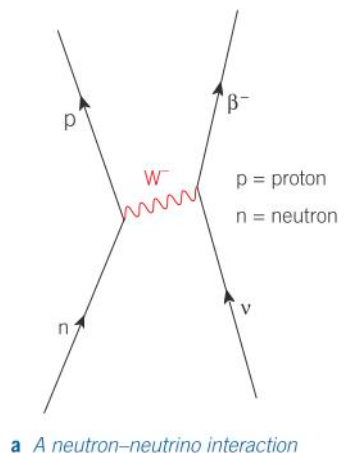
\includegraphics[width=6cm]{neutron-neutrino.png}
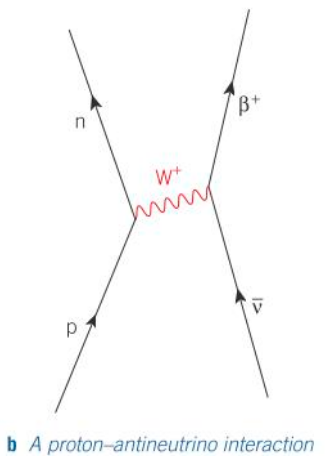
\includegraphics[width=6cm]{proton-antineutrino.png}
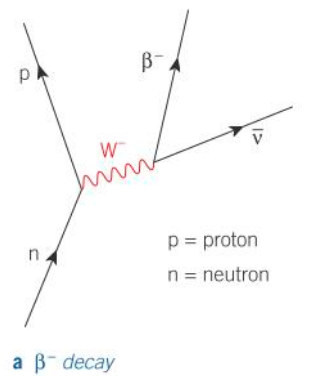
\includegraphics[width=6cm]{betaminus.png}
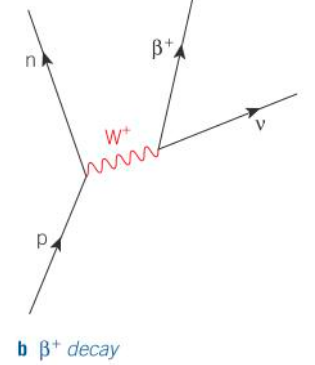
\includegraphics[width=6cm]{betaplus.png}
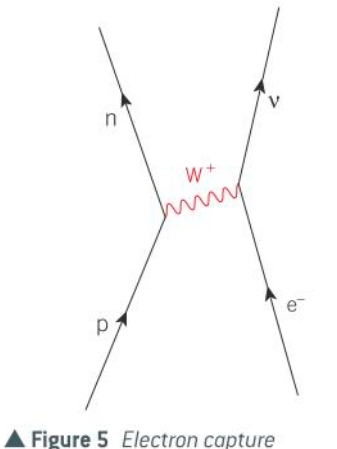
\includegraphics[width=6cm]{electron_capture.png}
\subsection{Classifications of particles}
{\renewcommand{\arraystretch}{2}
\begin{tabularx}{\textwidth}{|X|X|X|X|X|X|X|}
\hline
&\multicolumn{2}{|c|}{\centering Hadron}&\multicolumn{4}{|c|}{\centering Lepton}\\
\cline{2-7}
&Baryon&Meson&Electron&Muon&Electron neutrino&Muon neutrino\\
\hline
What it is&3 quarks&Quark antiquark pair&&&&\\
\hline
\end{tabularx}}
\paragraph{Baryons}
\begin{itemize}
\item Baryon number is conserved during interactions
\item The proton is the only stable baryon, all other baryons decay to it
\end{itemize}
\paragraph{Kaons and pions}
Kaons (K mesons) decay into Pions($\pi$ mesons), they decay by the weak interaction, so strangeness need not be conserved
$$K^+\rightarrow \mu^++\nu_\mu$$
$$K^+\rightarrow \pi^++\pi^0$$
$$K^-\rightarrow \mu^-+\overline{\nu_\mu}$$
$$K^-\rightarrow \pi^-+\pi^0$$
$$K^-\rightarrow \pi^0+\mu^-+\overline{\nu_\mu}$$
\paragraph{Leptons}
Lepton number is conserved in an interaction, muons decay into electrons
$$\mu^-\rightarrow e^-+\overline{\nu_e}+\nu_\mu$$
$$\mu^+\rightarrow e^++\nu_e+\overline{\nu_\mu}$$
\paragraph{Strange particles}
Strange particles are produced through the strong interaction and decay through the weak interaction, this is because strangeness is conserved during the strong interaction, but not during the weak interaction.
\subsubsection{Quarks and antiquarks}
Differences between quarks and antiquarks
\begin{itemize}
\item Opposite strangeness
\item Opposite charge
\item Opposite strangeness
\end{itemize}
\paragraph{Quark compositions}
\begin{itemize}
\item Proton -UUD
\item Neutron - DUD
\item Pion - Not strange, sign indicates charge
\item Kaon - Strange, sign indicates charge
\end{itemize}
\subsubsection{Applications of conservation laws}
Changes of quark nature
\begin{itemize}
\item $\beta^-$, down $\rightarrow$ up
\item $\beta^+$, up $\rightarrow$ down
\end{itemize}
\begin{center}
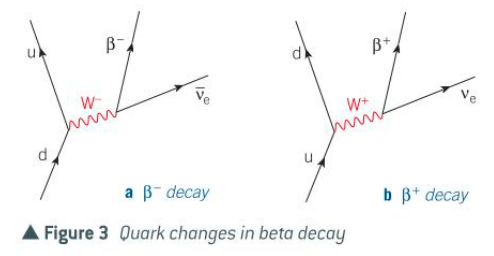
\includegraphics[width=10cm]{quark_beta.png}
\end{center}
In all interactions, energy and momentum must be conserved
\subsection{Electromagnetic radiation and quantum phenomena}
\subsubsection{The photoelectric effect}
\textbf{Photoelectric effect} - The emission of electrons from a metal surface when the surface is illuminated by a light of frequency greater than a minimum value known as the threshold frequency
\paragraph{Threshold frequency}
Because the energy of a photon is proportional to its frequency ($E=hf$), a minimum frequency must be reached so that the electrons have sufficient energy to escape the surface
\paragraph{Work function and stopping potential}
\textbf{Work function} - The minimum amount of energy needed by an electron to escape from a metal surface\\
\textbf{Stopping potential} - The potential difference required to stop an electron
\paragraph{The photoelectric equation}
$$hf=\phi+E_{K(Max)}$$
$hf$ is the energy of the incident photon\\
$\phi$ is the work function\\
$E_{K(max)}$ is the maximum kinetic energy\\
Electrons emitted will have a range of kinetic energies, depending how much work is done to escape the metal
\begin{tikzpicture}
\begin{axis}[axis lines=middle,scale=0.8,ylabel = KE,xlabel=Frequency,ylabel style={rotate=90,anchor=south},xlabel style={anchor=south},xmin=0,xmax=7,ymin=-5,ymax=7,xtick={2},xticklabels={$F_0$},ytick={-2},yticklabels={$-\Phi$}
]
\addplot[color=black,domain=0:7]{x-2};
\end{axis}
\end{tikzpicture}\\
The gradient of the line is Planck's constant
\subsubsection{Collisions of electrons with atoms}
\paragraph{Ionisation and excitation}
\textbf{Ion} - A charged atom\\
\textbf{Ionisation} - The process of creating ions\\
\textbf{Excitation} - The process in which an atom absorbs energy without becoming ionised as a result of an electron inside an atom moving from an inner shell to an outer shell
\paragraph{•}

\end{document}